\chapter{Introduction} 
% !TEX root = ../Almagest.tex

\section{Euclid's Elements and Ptolemy's Almagest}
The modern world inherited two major scientific treaties from the civilization
of ancient Greece. 
The first of these, the  {\em Elements}\/ (\begin{greek}Στοιχεῖα\end{greek}) of Euclid (\begin{greek}Εὐκλείδης\end{greek}), is a
large compendium of mathematical theorems concerning geometry, proportion, and number
theory. These theorems were not necessarily discovered by Euclid
himself---being largely the work of earlier mathematicians,
such as Eudoxos of Cnidus (\begin{greek}Εὔδοξος ὁ Κνίδιος\end{greek}), and Theaetetus of Athens (\begin{greek}Θεαίτητος ὁ Ἀθηναῖος\end{greek}) ---but were arranged
by him in a logical manner, so as to demonstrate that they can all ultimately
be derived from five simple axioms. The Elements is rightly regarded
as the first, largely successful, attempt to construct an
axiomatic system in mathematics, and is still held in high esteem within
the scientific community.

The second treatise, the {\em Almagest}\,\footnote{The true title
of this work is \begin{greek}Μαθηματικὴ Σύνταξις\end{greek}, which means ``Mathematical Treatise''.  The treatise was later called  \begin{greek}Ἡ Μεγάλη Σύνταξις\end{greek},  meaning ``The Great Treatise'',
and the superlative form of the adjective, \begin{greek}μεγίστη\end{greek},  with the Arabic article ``al" prepended, lies behind the Arabic name from which the English name Almagest derives.} of Claudius Ptolemy (\begin{greek}Κλαύδιος Πτολεμαῖος\end{greek}), 
is an attempt to find a simple geometric explanation for the apparent motions of the Sun,
the Moon, and the five visible planets in the Earth's sky.  On the basis of his own naked-eye observations, combined with those of earlier astronomers such as Hipparchus of Nicaea (\begin{greek}Ἱππάρχος ὁ Νικαεύς\end{greek}), Ptolemy proposed  a model of the Solar System in which the Earth is stationary.
According to this model, the Sun moves in a circular orbit, (nearly) centered on the Earth, that 
maintains a fixed inclination of about $23^\circ$ to the  terrestrial equator.
Furthermore, each planet moves  on the rim of a small
circle called an {\em epicycle}\/ (\begin{greek}ἐπίκυκλος\end{greek} in Greek), whose center revolves around the Earth
on a large eccentric circle called  a {\em deferent}\/ (\begin{greek}ἀποφορά\end{greek} in Greek). (See Figure~\ref{vf4}.) The
planetary deferents and epicycles also
maintain fixed inclinations,\footnote{Actually, Ptolemy erroneously allowed the inclinations of the
deferents and epicycles to vary slightly.} which are all fairly close to $23^\circ$,
to the  terrestrial equator. 

The scientific reputation of the Almagest has not fared  as well
as that of
Euclid's Elements. Nowadays, it is a commonly held belief, even amongst scientists,  that Ptolemy's mistaken adherence to the
 tenets of Aristotelian philosophy---in particular, the immovability of the Earth, and
 the necessity for heavenly bodies to move uniformly in circles---led him to
 construct an overcomplicated,  unwieldy, and faintly ridiculous model of planetary motion. As is well known, Ptolemy's model was superseded  in 1543 AD by the heliocentric model of 
 Nicolaus Copernicus, in which the planets revolve about the
 Sun in circular orbits.\footnote{In fact, the planets revolve on small circular epicycles, whose centers revolve around
 the Sun on eccentric circular deferents.} The Copernican model was, in turn,
 superseded in the early 1600's AD by the, ultimately correct, model
 of Johannes Kepler, in which the planets revolve about the Sun in eccentric 
 elliptical orbits.
 
 The aim of this treatise is to re-examine the scientific merits
 of Ptolemy's Almagest. 

 \section{Ptolemy's Model of the Solar System}
 Claudius Ptolemy lived and worked in the city of Alexandria, capital of the Roman
 province of Egypt, during the reigns of the later Flavian and 
 the Antonine emperors. Ptolemy was heir---via the writings of Euclid, and later mathematicians
 such as Apollonius of Perga (\begin{greek}Ἀπολλώνιος ὁ Περγαῖος\end{greek}), and Archimedes of Syracuse (\begin{greek}{Ἀρχιμήδης ὁ Συρακούσιος}\end{greek})---to the considerable mathematical
 knowledge of geometry and arithmetic acquired by the civilization of ancient Greece. Ptolemy
  also inherited an extensive ancient Greek tradition of observational and theoretical astronomy. The most important astronomer
 prior to Ptolemy was undoubtedly Hipparchus of Nicaea (second century BC), who developed the theory of solar motion used by Ptolemy, discovered
 the precession of the equinoxes, and collected  an extensive set of astronomical
 observations---some of which he made himself, and
 some of which dated back to Babylonian times---which were
 available to Ptolemy (possibly via the famous Library of Alexandria).
 Other astronomers who made significant contributions prior
 to Ptolemy include Meton of Athens (\begin{greek}Μέτων ὁ Ἀθηναῖος\end{greek}, 5th century BC),  Eudoxos of Cnidus (5th/4th century BC), Callipus of Cyzicus (\begin{greek}Καλλίππος ὁ Κυζίκιος\end{greek}, 4th century BC), Aristarchus of Samos (\begin{greek}Ἀρίσταρχος ὁ Σάμιος\end{greek}, 4th/3rd century BC),  
 Eratosthenes of Cyrene (\begin{greek}Ἐρατοσθένους τοῦ Κυρηναίου\end{greek}, 3rd/2nd century BC), and Menelaus
 of Alexandria (\begin{greek}Μενέλαος ὁ Ἀλεξανδρεύς\end{greek}, 1st century AD).
 
 Ptolemy's aim in the Almagest is to construct a kinematic model of
  the Solar System, as seen from the Earth. In other words, the Almagest outlines a relatively simple geometric model  that describes
 the apparent motions of the Sun, Moon, and planets, relative to the Earth, but does not attempt to explain
 why  these motions occur. (The models of Copernicus and Kepler are similar to that of Ptolemy in this respect.)  As such, the fact that the model described
 in the Almagest is geocentric in nature is a non-issue, because the Earth  is  stationary in its own frame of reference. This is not to say that the
 heliocentric hypothesis is without advantages. As we shall see, the
 assumption of heliocentricity allowed Copernicus to determine, for the first time, the ratios
 of the mean radii of the various planets in the Solar System.
 
 We now know, from the work of Kepler, that  planetary orbits are actually ellipses 
 that are confocal with the Sun. Such orbits possess two  main properties.
 First, they are eccentric; that is,  the Sun is displaced from the
 geometric center of the orbit. Second, they are elliptical; that is, 
  the orbit is elongated along a particular axis. Now, Keplerian orbits are  characterized by a quantity, $e$, know as the {\em eccentricity}, that 
 measures their deviation from circularity. It is easily demonstrated
 that the eccentricity of a Keplerian 
 orbit scales as $e$, whereas the corresponding degree of elongation
 scales as $e^2$. Because the orbits of the visible planets in the Solar System all possess relatively small values of $e$ (that is, $e\leq 0.21$), it follows that, to an excellent approximation, these orbits can be represented as eccentric circles; that is, 
 circles that are not quite concentric with the Sun. In other words,
 we can neglect the ellipticities of planetary orbits compared to
 their eccentricities.
 This is exactly
 what Ptolemy does in the Almagest.
 It follows that Ptolemy's
 assumption that heavenly bodies move in  circles  is actually
 one of the main strengths of his model, rather than 
 being the main weakness, as is commonly
 supposed.
 
 Kepler's second law of planetary motion states that the radius
 vector connecting a planet to the Sun sweeps out equal areas in equal
 time intervals. In the approximation in which planetary orbits
 are represented as eccentric circles, this law implies that a typical planet
 revolves around the Sun at a  non-uniform  rate. However,
 it is easily demonstrated  that the non-uniform rotation of the radius vector connecting the planet to the Sun  implies a  uniform rotation of the radius vector connecting the
 planet to the so-called {\em equant}; that is, the point diagrammatically opposite to the Sun
 with respect to the geometric center of the orbit. (See Figure~\ref{fsun}.)
 Ptolemy discovered the equant scheme empirically, and used it
 to control the non-uniform rotation of the planets in his model.
In fact,  this discovery is one of Ptolemy's main claims to fame.
 
It follows, from the previous discussion, that the geocentric model of Ptolemy is equivalent to a heliocentric
model in which the various planetary orbits are represented as
eccentric circles, and in which   the radius vector connecting a given planet
to its corresponding equant revolves at a  uniform rate. In fact, Ptolemy's
model of planetary motion can be thought of as a version of Kepler's model that 
is  accurate to  first order in the planetary eccentricities. (See Chapter~\ref{ckep}.)
According to the Ptolemaic scheme, from the point of view of the Earth,
the orbit of the Sun is described by a single circular motion, whereas
that of a planet is described by a combination of  two  circular motions. In reality, the single circular motion of the Sun 
represents the (approximately) circular motion of the Earth around the Sun,
whereas the two circular motions of a typical planet represent a combination of
the planet's (approximately) circular motion around the Sun, and the Earth's
 motion around the Sun. Incidentally, the popular myth that Ptolemy's
 scheme requires an absurdly large number of circles in order to
 fit the observational data to any degree of accuracy has no basis in fact. Actually,  Ptolemy's
 model of the Sun  and the planets, which fits the
 data very well, only contains 13 circles (that is, 6 deferents and 7 epicycles). (There are 7 epicycles because Mercury possesses an additional
 spurious epicycle.)

Ptolemy is often accused of slavish adherence to the tenants of  Aristotelian philosophy,
to the overall detriment of his model. However, despite Ptolemy's conventional geocentrism, his model of the Solar System deviates from orthodox 
Aristotelian philosophy in a number of crucially important respects. In his treatise \begin{greek}Περὶ Οὐρανοῦ\end{greek} (On the Heavens), 
Aristotle (\begin{greek}Ἀριστοτέλης\end{greek}) argues, from a purely philosophical standpoint, that
heavenly bodies should move in  single uniform circles.
However, in the Ptolemaic system, the motion of the planets is
a combination of  two  circular motions. Moreover, at least one
of these motions is non-uniform. Aristotle also argues, again
from purely philosophical grounds, that the Earth is located at the
exact center of the universe, about which all
heavenly bodies orbit in concentric circles.  However, in  the Ptolemaic system, the Earth is slightly displaced from the center of the universe. 
Indeed, there is no unique center of the universe, because the circular orbit
of the Sun and
the circular planetary deferents all have slightly different geometric centers,
none of which coincide with the Earth. As described in the Almagest, the non-orthodox
(from the point of view of Aristotelian philosophy) 
aspects of Ptolemy's model were ultimately dictated by  observations.
This suggests that, although Ptolemy's world-view was based on
Aristotelian philosophy, he did not hesitate to deviate from this standpoint
when required to by observational data.

From our heliocentric point of view, it is easily appreciated that the  epicycles 
of the  {\em superior planets}\/  (that is, the planets further from the Sun than
the Earth) in Ptolemy's model actually represent the Earth's  orbit around the Sun, whereas the
 deferents  represent the planets' orbits around the Sun. (See Figure~\ref{vf7}.)
It follows that the epicycles  of the superior planets should all be the  same size  (that is,
the size of the Earth's orbit), and that the radius vectors connecting
the centers of the epicycles to the planets should always all  point
in the  same direction  as the vector connecting the Earth to the Sun.

We can also appreciate that the  deferents  of the  {\em inferior 
planets}\/ (that is, the planets closer to the Sun than
the Earth) in Ptolemy's model actually represent the  Earth's orbit around the Sun, whereas the
 epicycles  represent the planets'  orbits around the Sun.  (See Figure~\ref{vf8}.)
It follows that the  deferents of the inferior planets should all be the
same size (that is, the size of the Earth's orbit), and that the
centers of the epicycles (relative to the Earth) should all correspond to the position of the Sun (relative to the Earth). 

\begin{figure}
\centerline{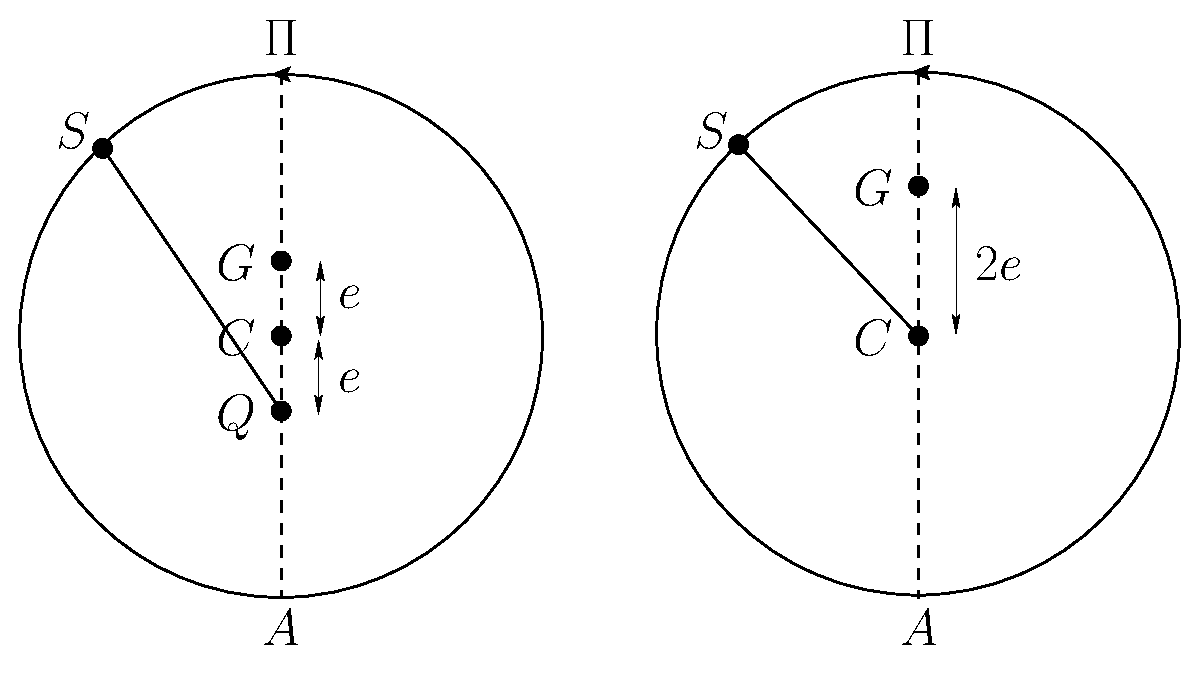
\includegraphics[height=3in]{epsfiles/sun.eps}}
\caption{Hipparchus' (and Ptolemy's) model of the Sun's apparent orbit  about the Earth (right) compared to the optimal  model (left).  The
radius vectors in both models rotate uniformly. Here, $S$ is the Sun, $G$ the Earth, $C$ the geometric center of the orbit, $Q$ the equant, $\Pi$ the perigee, and $A$ the apogee. The radius of the orbit is normalized to unity.}\label{fsun}   
\end{figure}

The geocentric model of the Solar System outlined previously represents a perfected version
of Ptolemy's model, constructed with 
a knowledge of the true motions of the planets around the Sun.
Not surprisingly, the  model actually described in the Almagest deviates
somewhat from this ideal form. In the following, we shall
refer to these deviations as ``errors'', but this should not be understood
in a pejorative sense.

Ptolemy's first error lies in his model of the Sun's apparent motion around the Earth, which he inherited
from Hipparchus. Figure~\ref{fsun} compares what Ptolemy actually
did, in this respect, compared to
what he should have done in order to be completely consistent
with the rest of his model. Let us normalize the mean radius of the Sun's
apparent orbit  to unity, for the sake of clarity.
 Ptolemy should
have adopted the model shown on the left in Figure~\ref{fsun}, in which the Earth
is displaced from the center of the Sun's orbit a distance $e=0.0167$ (the eccentricity of the Earth's orbit around the Sun) towards the perigee (the point of the Sun's closest approach
to the Earth), and the equant is displaced the same distance in the opposite
direction. The instantaneous angular position of the Sun is then obtained
by allowing the radius vector connecting the equant to the Sun to rotate uniformly at the Sun's mean orbital angular velocity. Of course, this implies that the
Sun rotates non-uniformly about the Earth. Ptolemy actually adopted the Hipparchian model
shown on the right in Figure~\ref{fsun}. In this model, the Earth is displaced
a distance $2e$ from  the center of the Sun's orbit in the direction of the perigee,
and the Sun rotates at a uniform rate (that is, the radius vector $CS$ rotates uniformly). It turns out that, to first order in $e$, these two
models are equivalent in terms of their ability to predict the angular position of the Sun relative to the Earth. (See Chapter~\ref{ckep}.) Nevertheless, the Hipparchian
model is incorrect, because it predicts too large (by a factor of two) a variation in  the radial distance of the Sun from the Earth (and, hence,  the angular size of the Sun)  during the
course of a year. (See Chapter~\ref{ckep}.) Ptolemy probably adopted
the Hipparchian model because his Aristotelian leanings prejudiced him in favor of uniform circular motion whenever this was consistent with observations.
(It should be noted that Ptolemy was not  interested in explaining the relatively small variations in the angular size of the Sun during the year; presumably, because this effect would have been very difficult for him to accurately measure.)

Ptolemy's next error was to neglect the non-uniform rotation of the
superior planets on their epicycles. This is equivalent to neglecting
the orbital eccentricity of the Earth (recall that the epicycles of the superior
planets actually represent the Earth's orbit) compared to those of
the superior planets. It turns out that this is a fairly good approximation,
because the superior planets all have significantly greater orbital eccentricities
than the Earth. Nevertheless, 
neglecting  the non-uniform rotation of the
superior planets on their epicycles has the unfortunate effect of obscuring the tight coupling between
the apparent motions of these planets, and that of the Sun. The radius vectors connecting the epicycle centers of the
superior planets to the planets themselves should always all point  exactly in the
same direction as that of the Sun relative to the Earth.
When the aforementioned non-uniform rotation is neglected, the radius
vectors instead point in the direction of the  mean Sun  relative to
the Earth. The {\em mean Sun}\/ is a fictitious body that has the
same apparent orbit around the Earth as the real Sun, but that circles
the Earth at a uniform rate. The mean Sun only coincides with the
real Sun twice a year.

Ptolemy's third error is associated with his treatment of the
inferior planets. As we have seen, in going from the superior to the
inferior planets, deferents and epicycles effectively swap roles. 
For instance, it is the deferents  of the inferior planets, rather than the epicycles, that represent
the Earth's orbit. Hence, for the sake of consistency with his treatment of
the superior planets, Ptolemy should have neglected the non-uniform
rotation of the epicycle centers around the deferents of the inferior
planets, and retained the non-uniform rotation of the planets themselves around the
epicycle centers. Instead, he did exactly the opposite. This
is equivalent to neglecting the inferior planets' orbital eccentricities relative to
that of the Earth. It follows that this approximation only works when an inferior
planet has a significantly smaller  orbital eccentricity than that of the Earth.
It turns out that this is indeed the case for Venus, which has the smallest eccentricity
of any planet in the Solar System. Thus, Ptolemy was able to
successfully account for the apparent motion of Venus. Mercury, on the
other hand, has a much larger orbital eccentricity than the Earth. Moreover, it
is particularly difficult to obtain good naked-eye positional data for Mercury, because this planet always appears 
very close to the Sun in the sky. Consequently,
Ptolemy's Mercury data was highly inaccurate.
 Not surprisingly, Ptolemy was not able to account for the apparent motion of Mercury
using his standard deferent-epicycle approach. Instead, in order to fit the data, he was forced
to introduce an additional, and entirely spurious, epicycle into his  model of
Mercury's orbit.

Ptolemy's fourth, and possibly largest, error is associated with his treatment
of the Moon. It should be noted that the Moon's motion around the
Earth is extremely complicated in nature, because it is strongly perturbed by the Sun,  and was not fully understood until
the early 20th century AD. Ptolemy constructed an ingenious geometric
model of the Moon's orbit that was capable of predicting
the lunar ecliptic longitude to reasonable accuracy. Unfortunately, this
model necessitates a monthly variation in the Earth-Moon distance  by a factor of about two, 
which  implies a similarly large variation in the Moon's angular diameter. However, the observed variation in the   Moon's diameter is very much smaller than this. Hence, Ptolemy's model of lunar motion is not even approximately correct.

Ptolemy's fifth error is associated with his treatment of planetary
ecliptic latitudes. Given that the deferents and epicycles of
the superior planets represent the orbits of the planets themselves around the
Sun, and the Sun's apparent orbit around the Earth, respectively, it follows
that one should take the slight inclination of planetary orbits to
the ecliptic plane (that is, the plane of the Sun's apparent orbit)
into account by tilting the deferents of superior planets, while keeping their epicycles
parallel to the ecliptic. Similarly, given that the epicycles and deferents of
inferior planets represent the orbits of the planets themselves around the
Sun, and the Sun's apparent orbit around the Earth, respectively, one should tilt the epicycles of
inferior planets, while keeping their deferents parallel to the ecliptic. 
Finally, because the inclination of  planetary orbits are all essentially constant in time, the inclinations
of the epicycles and deferents should also be constant. 
Unfortunately, when Ptolemy constructed his theory of
planetary latitudes, he tilted  the both deferents and epicycles of
all of the planets. Even worse, he allowed the inclinations of the epicycles to
the ecliptic plane to vary in time. The net result is a theory which is far more
complicated than is necessary.

The final failing in Ptolemy's model of the Solar System lies in its  scale invariance. 
Using angular position data alone, Ptolemy was  able to determine the ratio 
of the epicycle radius to that of the deferent for each planet, but was
not able to determine the  relative sizes  of the deferents of different planets. 
In order to break this scale invariance it is necessary to make an
additional assumption; namely, that the Earth orbits the Sun. This
brings us to Copernicus.

\section{Copernicus's Model of the Solar System}
The Polish astronomer Nicolaus Copernicus (1473--1543 AD) studied the
Almagest assiduously, but eventually became dissatisfied with
Ptolomy's approach. The main reason for this dissatisfaction was
not the geocentric nature of Ptolomy's model, but rather the fact that it
mandates that heavenly bodies  execute non-uniform circular
motion. Copernicus, like Aristotle, was convinced that the supposed perfection
of the heavens requires  such bodies to execute uniform  circular motion only. Copernicus was thus spurred to construct his own
model of the Solar System, which was described in his book {\em De Revolutionibus Orbium Coelestium}\/ (On the Revolutions of the Heavenly Spheres), published in the year of his death.

The most well-known aspect of Copernicus's model is the fact that it
is  heliocentric. As has already been mentioned, when describing
the motion of the Sun, Moon, and planets relative to the Earth, it makes
little practical difference whether one adopts a geocentric or a heliocentric
model of the Solar System. Having said this, the heliocentric approach does have one large advantage. If we accept that the Sun,  and not the Earth,
is stationary, then it immediately follows that the epicycles of the
superior planets, and the deferents of the inferior planets,  represent the Earth's orbit around the Sun. Hence, all of these circles
must be the same size. This realization allows us to break the
scale invariance which is one of the main failings of Ptolemy's
model. Thus, the ratio of the deferent radius to that of the
epicycle for a superior planet, which is easily inferred from observations,
actually corresponds to the ratio of planet's orbital radius to that of the
Earth. Likewise, the ratio of the epicycle radius to that of the deferent
for an inferior planet, which is again easily determined observationally, also corresponds to the ratio of the planet's
orbital radius to that of the Earth. Using this type of reasoning,
Copernicus was able to construct the first accurate scale model
of the Solar System, and to firmly establish the order in which the planets
orbit the Sun. In some sense, this was his main achievement.

Copernicus's insistence that heavenly bodies should only move in uniform 
circles lead him to reject Ptolemy's  equant scheme, and to  replace
it with the scheme illustrated in Figure~\ref{fplan}. According to Copernicus, a heliocentric
planetary orbit is a combination of  two  circular motions. The first is 
the motion of the planet around a small circular epicycle, and the second is the motion of the center of
the epicycle around the Sun on  a circular deferent. Both motions are  uniform, and in the same direction.
However, the former motion is twice as fast as the latter. In addition, the Sun is displaced
from the center of the deferent in the direction of the perihelion, the displacement being
proportional to the orbital eccentricity. Furthermore, the Sun's displacement
is  three  times greater than the radius of the epicycle. Finally, the
radius of the deferent is equal to the major radius of the planetary orbit. It turns
out that Copernicus' scheme is a marginally less accurate approximation  than Ptolemy's to 
a low eccentricity Keplerian orbit. (See Chapter~\ref{ckep}.) 

Copernicus modeled the
orbit of the Earth around the Sun using an Hipparchian scheme (see Figure~\ref{fsun}) in which the Earth moves
uniformly around an eccentric circle.  Unfortunately, such a scheme exaggerates the variation in the
radial distance between the Earth and the Sun during the course of a year by a factor of two, and so
introduces significant errors into the calculation of the parallax of the planets due to the motion of the Earth. 
On the other hand, Copernicus' model of the Moon's orbit around the Earth is a considerable improvement on Ptolemy's, because
it does not grossly exaggerate the monthly variation in the Earth-Moon distance. 
Like Ptolemy, Copernicus  introduced an additional spurious epicycle into his model
of Mercury's orbit, and erroneously allowed the
inclination of his planetary orbits to vary slightly  in time. 

In summary, Copernicus's model of the Solar System contains approximately the 
 same number of epicycles as Ptolemy's, the only difference being that Copernicus' epicycles are much 
 smaller than Ptolemy's.  Indeed, the model of Copernicus is about as complicated, and not appreciably more accurate, than that described in the  Almagest. 
In this respect, Copernicus cannot be said to have demonstrated
the correctness of his heliocentric approach on the basis of observational data. 

\begin{figure}
\centerline{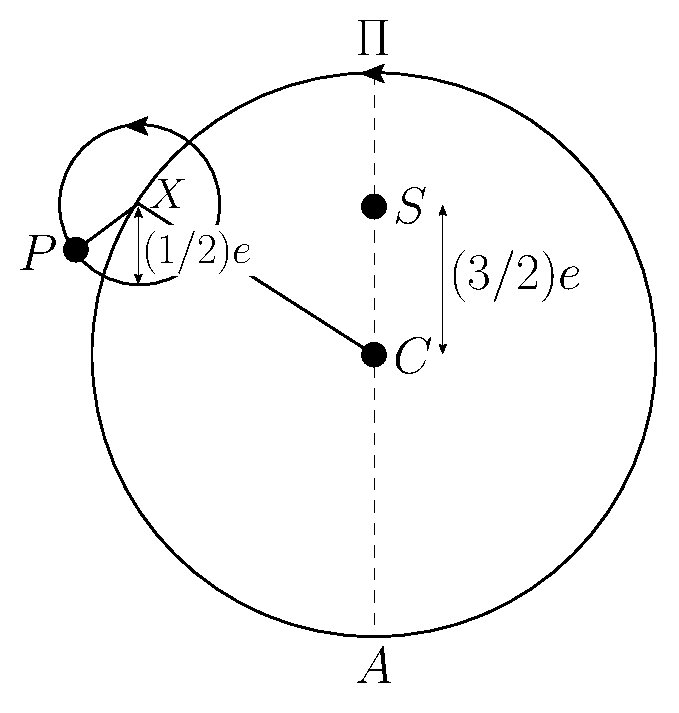
\includegraphics[height=3in]{epsfiles/fig1.2x.eps}}
\caption{Copernicus' model of a heliocentric planetary orbit. Here, $S$ is the Sun, $P$ the planet, $C$ the geometric center of the deferent, $X$ the center of the epicycle, $\Pi$ the perihelion, and $A$ the aphelion. The radius vectors $CX$ and $XP$ both rotate uniformly in the
same direction,
but $XP$ rotates twice as fast as $CX$. The major radius of the orbit is normalized to unity.}\label{fplan}   
\end{figure}

\section{Kepler's Model of the Solar System}
Johannes Kepler (1571--1630 AD) was fortunate  to inherit an extensive set of naked-eye solar, lunar, and planetary angular position data
 from the Danish astronomer Tycho Brahe (1546--1601 AD). This data
 extended over many decades, and was of unprecedented accuracy.
 
 Although Kepler adopted the heliocentric approach of Copernicus,
 what he effectively first did was to  perfect Ptolemy's model of the Solar System (or, rather,
 its heliocentric equivalent). Thus, Kepler replaced Ptolemy's
 erroneous equantless model of the Sun's apparent orbit around the
 Earth with a corrected version containing an equant; in the process,
 halving the eccentricity of the orbit. (See Figure~\ref{fsun}.)  Kepler also introduced equants
 into the epicycles of the superior and inferior planets. Once he had perfected Ptolemy's model, the heliocentric nature of
 the Solar System became manifestly apparent to Kepler. For instance,
 he found that the epicycles of the superior planets, the Sun's
 apparent orbit around the Earth, and the deferents of the inferior
 planets, all had exactly the  same eccentricity. The obvious implication
  is that these circles all correspond to some common motion within the
 Solar System; in fact, the motion of the Earth around the Sun.
 
 Once Kepler had corrected the Almagest model, he compared its predictions
 with his observational data. In particular, Kepler investigated 
 the apparent motion of Mars in the night sky. Kepler found that his  model performed extremely well,
 but that there remained small differences between its predictions and the observational data. The maximum discrepancy was about $8'$; that is, about one
 quarter of the apparent size of the
 Sun. By the standards of naked-eye astronomy, this was a very small discrepancy. Nevertheless, given the incredible accuracy of Tycho Brahe's
 observations, the discrepancy was still significant. Thus, Kepler embarked on an epic new series
 of calculations which eventually lead him to the conclusion that the
 planetary orbits are actually eccentric ellipses, rather than eccentric circles. 
 Kepler published the results of his research in  his treatise {\em Astronomia Nova}\/ (New Astronomy) in 1609 AD.
 It is
 interesting to note that had Tycho's data been a little less accurate,
 or had the orbit of Mars been a little less eccentric, Kepler might well 
 have settled for a model which was kinematically equivalent to
 a perfected version of the model described in the Almagest. We can also
 appreciate that, given the far less accurate observational data available to
 Ptolemy, there was no way in which he could have discerned the
 very small difference between elliptical planetary orbits and the eccentric
 circular orbits employed in the Almagest.
 
 \section{Purpose of Treatise}
As we have seen, misconceptions abound regarding the details of Ptolemy's model of the Solar System, as well as  its scientific merit. Part of the reason for this is 
that the Almagest is an extremely difficult book for a
modern reader to comprehend.  For instance, virtually all of its theoretical results are justified via lengthy  and opaque geometric
proofs. Moreover, the  plane and
spherical trigonometry employed by Ptolemy is of a rather primitive  nature, and,
consequently, somewhat unwieldy. Dates are also a major stumbling block, because three different systems are used in the Almagest,
all of which are archaic, and essentially meaningless to the modern reader.
Another difficulty is the unfamiliar, and far from optimal, ancient Greek method of representing numbers and fractions.
Finally, the terminology employed in the Almagest is, in many instances, significantly different to that used in modern
astronomy textbooks.

The aim of this treatise is to reconstruct Ptolemy's model of the Solar System employing
modern  mathematical methods, standard dates, and conventional astronomical terminology. It
is hoped that the resulting model will enable the reader to comprehend the full extent of Ptolemy's scientific
achievement. In fact, the model described
in this work is a somewhat improved version of Ptolemy's, in that
all of the  previously mentioned deficiencies   have been corrected. Furthermore, Ptolemy's equant scheme has been replaced by a Keplerian scheme, expanded to second order in the planetary
eccentricities.
It should be noted, however, that these two schemes are essentially indistinguishable for
small eccentricity orbits. 
Certain aspects of the Almagest have not been reproduced. For instance, it was not thought necessary to instruct the reader on how to construct
trigonometric tables, or primitive astronomical instruments. Furthermore, no attempted has been made to derive any of the model parameters directly from
 observational data, because the orbital elements and physical properties of the Sun, Moon, and planets are, by now, extremely well established. Any detailed discussion of the fixed stars has also been omitted, because stellar positions  are also very well established, and the apparent motion
 of the stars in the sky is comparatively straightforward compared to those of the Sun, the Moon, and the planets. 
 What remains is a mathematical model of the Solar
 System that is surprisingly accurate (the maximum errors in the ecliptic
 longitudes of the Sun, Moon, Mercury, Venus, Mars, Jupiter, and
 Saturn during the years 1995--2006 AD are $0.7'$, $14'$, $28'$, $10'$,
 $14'$, $4'$, and $1'$, respectively), yet sufficiently simple that all of the
 necessary calculations can be performed by hand, with the aid of tables. The form of the calculations, as well as the layout of the tables,
 is, for the most part, fairly similar to those found in the Almagest. Many examples
 of the use of the tables are provided. 
